
\section{Pewarisan (Inheritance)}\label{pewarisan-inheritance}

Pemrograman Berorientasi Objek mempunyai fitur penting yang memudahkan
pemrogram dalam membuat program yaitu pewarisan (inheritance). Aspek
penting pewarisan dalam pemrograman berorientasi objek adalah pemakaian
kode program yang sudah ada (code reuse), yang akan dibahas pada bab ini
dan polimorfisme (polymorhism) yang akan dibahas pada bab berikutnya.
Kelas yang sudah ada dapat digunakan lagi untuk dikembangkan menjadi
kelas yang baru, dalam hal ini kelas yang sudah ada dinamakan kelas
dasar (base class) sedang kelas baru yang akan dibuat dinamakan kelas
turunan (derived class). Dengan demikian, semua anggota kelas dasar yang
tidak bersifat privat akan diwarisi oleh kelas turunannya dan pemrogram
tinggal menambahkan anggota-anggota baru untuk menambahkan
fungsionalitas kelas tersebut.

\section{Penulisan Penurunan}\label{penulisan-penurunan}

Untuk membuat kelas turunan dapat dilakukan dengan cara sama seperti
mendeklarasikan kelas biasa dengan menambahkan titik dua (:) setelah
nama kelas dan diikuti dengan jenis penurunan (public dsb.) dan nama
kelas dasar yang akan diturunkan, bentuk umum adalah seperti berikut:

\begin{lstlisting}[language=c++, numbers=none]
class <kelas_turunan> : <jenis_penurunan> <kelas_dasar>
\end{lstlisting}

Sebagai contoh misalnya akan dibuat kelas turunan Silinder dari kelas
dasar Lingkaran, maka dapat dituliskan :

\begin{lstlisting}[language=c++, numbers=none]
class Silinder : public Lingkaran
\end{lstlisting}

Mengenai jenis akses public ini akan dibahas nanti, sekarang kita akan
memakai public. Kelas dasar yang akan diturunkan harus sudah
dideklarasikan lebih dahulu, jika tidak maka kita akan menjumpai pesan
kesalahan kompiler.

\subsubsection*{Contoh Pewarisan (Inheritance).}

Buka Qt Creator dan buat project Qt Console Application baru dengan nama
Contoh \ref{Pewarisan-Inheritance}, kemudian tulis kode berikut.

\begin{lstlisting}[language=c++, caption=Pewarisan (Inheritance), label=Pewarisan-Inheritance]
#include <QtCore/QCoreApplication>
#include <iostream>
using namespace std;
class Lingkaran{
public:
//Konstruktor
Lingkaran(float radius = 0){
Lingkaran::radius = radius;
}
//Destruktor
    ~Lingkaran(){}
protected :
float radius;
public :
float getLuas(){
return 3.14 * radius * radius;
}
};
class Silinder : public Lingkaran{
public:
//Konstruktor
Silinder(float radius, float tinggi){
Silinder::radius = radius; //<-- warisan
Silinder::tinggi = tinggi; //<-- anggota baru
}
//Destruktor
~Silinder(){}
private:
float tinggi; //<-- anggota baru
public:
float getVolume(){ //<-- anggota baru
//getLuas() adalah warisan
return getLuas() * tinggi;
}
};
int main(int argc, char *argv[])
{
QCoreApplication a(argc, argv);
Silinder drum(50,125);
cout << "Volume drum = " << drum.getVolume() << " Cm2" << endl;
return a.exec();
}
\end{lstlisting}

Kemudian jalankan kode di atas dengan menekan tombol Ctrl+R, outputnya
adalah sebagai berikut.

\begin{lcverbatim}
Volume drum = 981250 Cm2
\end{lcverbatim}

\textbf{Keterangan Program :}

\begin{itemize}

\item
  Pada program diatas sudah dibuat kelas \texttt{Lingkaran}, dengan
  variabel anggota \texttt{radius} bertipe \texttt{float} dan fungsi
  anggota \texttt{getLuas()} yang mengembalikan nilai \texttt{float}.
\item
  Kelas kedua adalah \texttt{Silinder} yang merupakan turunan dari kelas
  \texttt{Lingkaran}, oleh karena itu deklarasi dituliskan :
  \texttt{class\ Silinder\ :\ Lingkaran}, dengan demikian kelas
  \texttt{Silinder} akan mewarisi anggota kelas \texttt{Lingkaran} yang
  tidak private, yaitu : variabel anggota \texttt{radius} bertipe
  \texttt{float} dan fungsi anggota \texttt{getLuas()} yang mengemalikan
  nilai \texttt{float}.
\item
  Tampak pada kelas \texttt{Silinder} ditambahkan variabel anggota
  tinggi bertipe \texttt{float} dan fungsi anggota \texttt{getVolume()}
  yang mengembalikan nilai \texttt{float}. Ini memberikan contoh
  penambahan fungsionalitas dari kelas yang sudah ada.
\item
  Pada fungsi anggota \texttt{getVolume()} pada kelas \texttt{Silinder},
  nilai kembalian dirumuskan \texttt{return\ getLuas()\ *\ tinggi}, ini
  menjelaskan bahwa fungsi \texttt{getLuas()} tersebut sekarang juga
  menjadi milik kelas \texttt{Silinder} (\emph{mendapat warisan}).
\item
  Pada hasil eksekusi, tampak bahwa fungsi \texttt{getVolume()}
  menghitung \emph{(3.14 * 50 * 50 )* 125} dan menghasilkan nilai
  981250. Ini berarti perhitungan \texttt{getLuas()} memakai fungsi
  anggota milik kelas Lingkaran yang diwariskan kepada kelas Silinder.
\end{itemize}

\section{Jenis Akses Penurunan
Kelas}\label{jenis-akses-penurunan-kelas}

Deklarasi kelas Silinder di atas adalah :
\texttt{class\ Silinder\ :\ public\ Lingkaran}, ini berarti semua
anggota yang bersifat \texttt{public} dan \texttt{protected} dari kelas
\texttt{Lingkaran} akan diwariskan kepada kelas \texttt{Silinder} dan
pada kelas \texttt{Silinder} anggota-anggota warisan tersebut akan tetap
mempunyai jenis akses seperti itu. Namun jika modifier akses public
dihilangkan maka berarti pewarisan memakai jenis akses private, sebab
secara default C++ memakai jenis akses private jika modifer akses tidak
dituliskan. Jika ini terjadi, maka akan terjadi perubahan modifier akses
terhadap anggota-anggota warisan tersebut di dalam kelas Silinder, yaitu
semua anggota yang diwariskan (baik berjenis public maupun protected)
akan berubah menjadi private di dalam kelas Silinder.

\subsubsection*{Contoh  Jenis Akses Public Pada Penurunan.}

Buka project Contoh \ref{Pewarisan-Inheritance} di atas, kemudian tambahkan (edit) kode berikut
pada fungsi
\texttt{main()\ :\ cout\ \textless{}\textless{}\ "Milik\ Base\ Class\ -\/-\textgreater{}\ "\ \textless{}\textless{}\ drum.getLuas()\ \textless{}\textless{}\ endl;}

\begin{lstlisting}[language=c++, caption=Jenis Akses Public Pada Penurunan, label=]
int main(int argc, char *argv[])
{
QCoreApplication a(argc, argv);
Silinder drum(50,125);
cout << "Milik Base Class --> " << drum.getLuas() << endl;
cout << "Volume drum = " << drum.getVolume() << " Cm2" << endl;
return a.exec();
}
\end{lstlisting}

Kemudian jalankan kode di atas dengan menekan tombol Ctrl+R, outputnya
adalah sebagai berikut.
\begin{lcverbatim}
Volume drum = 981250 Cm2
Milik Base Class --> 7850
\end{lcverbatim}


\textbf{Keterangan Program :}

Tampak pada program dapat mengakses metode warisan kelas Lingkaran dari
dalam program utama (main()). Ini menunjukkan bahwa metode tersebut
diwariskan ke kelas Silinder dan jenis aksesnya masih tetap sama yaitu
public.

Kemudian hapuslah jenis akses penurunan public (atau gantilah dengan
private) pada deklarasi kelas Silinder yang tadinya:

\begin{lstlisting}[language=c++, numbers=none]
class Silinder : public Lingkaran
\end{lstlisting}

Sehingga menjadi:

\begin{lstlisting}[language=c++, numbers=none]
class Silinder : Lingkaran
\end{lstlisting}

Kemudian jalankan kode diatas dengan menekan tombol Ctrl+R, maka tidak
akan ada output karena terjadi kesalahan kompilasi sebagai berikut.

\begin{figure}[htbp]
\centering
\includegraphics[width=0.8\textwidth]{images/capture7-1.png}

\end{figure}

\textbf{Keterangan Program :}

Tampak pada program metode warisan kelas Lingkaran bernama getLuas()
tidak dapat diakses dari dalam program utama (main()). Hal ini
disebabkan karena metode tersebut ketika diwariskan ke kelas Silinder
jenis aksesnya berubah menjadi private, yang berarti diwariskan akan
tetapi hanya dapat diakses dari dalam kelas Silinder, akibatnya ketika
akan diakses dari program utama (main()), terjadi kesalahan kompilasi
seperti di atas.

Berikut ini adalah perubahan jenis akses anggota dari kelas dasar ke
kelas turunan berdasarkan jenis akses penurunan:

\begin{quotation}
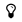
\includegraphics{images/tips}	\textbf{TIPS} 
	
	Pada
	umumnya jenis akses penurunan adalah \emph{public}, oleh karena itu
	biasakan menuliskan jenis akses public ketika akan menurunakan suatu
	kelas.
\end{quotation}
 

\section{Warisan}\label{warisan}

Anggota-anggota kelas (member variable dan member function) mempunyai
jenis akses private, protected dan public, jika tidak dituliskan pada
deklarasi anggota tersebut maka akan digunakan jenis akses private.
Dalam hal pewarisan (inheritance) pada pemrograman berorientasi objek,
seperti sudah dijelaskan di atas bahwa anggota yang diwariskan adalah
anggota dengan jenis akses public atau protected. Jenis akses public
pada suatu anggota artinya bahwa anggota tersebut dapat diakses dari
manapun dan akan diwariskan jika kelas tersebut diturunkan, sedangkan
jenis akses protected berarti anggota tersebut diwariskan kepada kelas
turunannya dan hanya bisa diakses dari dalam kelas turunan tersebut.
Berikut ini adalah tabel yang menjelaskan jenis akses dan aksesibilitas
suatu anggota:

\begin{longtable}[]{@{}llll@{}}
\toprule
Aksesibilitas & public & protected & private\tabularnewline
\midrule
\endhead
Dari dalam kelas itu sendiri & Ya & Ya & Ya\tabularnewline
Dari kelas beda turunan & Ya & Ya & Tidak\tabularnewline
Dari kelas beda tetapi bukan turunan & Ya & Tidak & Tidak\tabularnewline
\bottomrule
\end{longtable}

Perlu diketahui bahwa konstruktor dan destruktor tidak diwariskan. Hal
ini bisa dimaklumi, sebab konstruktor bekerja spesifik untuk kelas
tersebut. Pada C++ jelas bahwa nama konstruktor sama dengan nama
kelasnya, karena nama kelas turunan tidak mungkin sama dengan nama kelas
dasar, maka tidak mungkin konstruktor kelas dasar juga merupakan
konstruktor kelas turunan.

Namun demikian, pada konteks pewarisan, perlu diketahui bahwa itu tidak
berarti konstruktor kelas dasar dapat diabaikan, sebab bagaimanapun juga
dalam pembentukan objek konstruktor suatu kelas pasti bekerja (oleh
karena itu diberi nama ``konstruktor'' yang artinya pembentuk). Berikut
ini hal-hal yang perlu diperhatikan pada pewarisan mengenai konstruktor:

\subsection{Tiap Kelas Mempunyai
Konstruktor}\label{tiap-kelas-mempunyai-konstruktor}

Tidak ada kelas yang tidak mempunyai konstruktor. Adalah benar bahwa
secara eksplisit kita bisa menuliskan sebuah kelas tanpa mendeklarasikan
konstruktor sama sekali, namun itu tidak berarti bahwa kelas tersebut
tidak mempunyai kontruktor, sebab sebenarnya yang dieksekusi oleh
komputer bukan kode program yang kita tulis tersebut, melainkan hasil
kompilasi dari kode program tersebut. Pada waktu dikompilasi, kompiler
akan menambahkan konstruktor tanpa parameter yang tidak melakukan
apa-apa seperti berikut:

\begin{lstlisting}[language=c++, numbers=none]
<nama_kelas>(){}
\end{lstlisting}

\subsubsection*{Contoh  Konstruktor default.}

\begin{enumerate}

\item
  Buka Qt Creator, buat project Qt Console Application dengan nama
  Contoh \ref{Konstruktor-default}. Kemudian tulis kode berikut.

\begin{lstlisting}[language=c++, caption=Konstruktor default, label=Konstruktor-default]
#include <QtCore/QCoreApplication>
#include <iostream>
using namespace std;
class Kelasku{
public:
Kelasku(){} //<-- konstruktor ini boleh tidak ditulis
public:
    void hai(){
cout << "Hai, apa khabar...?" << endl;
}
};
int main(int argc, char *argv[])
{
QCoreApplication a(argc, argv);
Kelasku test;
test.hai();
return a.exec();
}
\end{lstlisting}
\item
  Tekan Ctrl+R untuk menjalankan kode di atas, outputnya adalah sebagai
  berikut.

\begin{lcverbatim}
 Hai, apa khabar...?
\end{lcverbatim}



\item
  Kemudian hapuslah konstruktor \texttt{Kelasku()\{\}}, kemudian tekan
  Ctrl+R untuk menjalankan kode di atas, outputnya adalah sebagai
  berikut.
  \begin{lcverbatim}
  Hai, apa khabar...?
  \end{lcverbatim}
\end{enumerate}



\textbf{Keterangan Program:}

Pada contoh program ini tampak bahwa ada konstruktor maupun tidak ada
konstruktor program di atas tetap bisa dijalankan dan tidak ada
perbedaan sama sekali. Hal ini disebabkan oleh karena jika suatu kelas
tidak mempunyai kontruktor, maka secara otomatis kompiler akan
menambahkan konstruktor default (yaitu konstruktor tanpa parameter dan
tanpa program apapun) pada hasil kompilasi, jadi pada contoh program di
atas hasil kompilasi dengan atau tanpa konstruktor adalah tetap sama.

\subsection{Konstruktor Kelas Turunan Pasti Memanggil Konstruktor
Kelas
Dasar}\label{konstruktor-kelas-turunan-pasti-memanggil-konstruktor-kelas-dasar}

Seperti dijelaskan di atas bahwa tidak ada kelas yang tidak mempunyai
konstruktor, demikian juga dengan kelas turunan. Pada waktu ada
pembentukan suatu objek dari suatu kelas turunan, secara otomatis ada
terlebih dahulu pembentukan objek kelas dasarnya karena harus ada
anggota-anggota yang diwariskan, dengan demikian bisa dimengerti bahwa
konstruktor kelas turunan pasti memanggil konstruktor kelas dasarnya.

Sama seperti pada penulisan kelas biasa, pada kelas turunan juga bisa
tidak dituliskan konstruktor secara eksplisit dan pada kasus ini pada
saat kompilasi kompiler akan menambahkan konstruktor kosong tanpa
parameter. Namun bentuk konstruktor kosong pada kelas turunan berbeda
dengan konstruktor kosong kelas biasa, karena pada konstruktor kosong
kelas turunan akan memanggil konstruktor kosong kelas dasarnya.

\subsubsection*{Contoh Konstruktor default kelas turunan.}

\begin{enumerate}

\item
  Buka Qt Creator, buka project Qt Console Application dengan nama
  Contoh \ref{Konstruktor-default} tadi. Kemudian ubah isi konstruktor kelas Kelasku dan
  tambahkan kelas Turunan berikut.

\begin{lstlisting}[language=c++, caption=Konstruktor default kelas turunan, label=Konstruktor-default-kelas-turunan]
#include <QtCore/QCoreApplication>
#include <iostream>
using namespace std;
class Kelasku{
public:
Kelasku(){
cout << "Konstruktor Kelas Dasar dijalankan..." << endl;
}
public:
void hai(){
cout << "Hai, apa khabar...?" << endl;
}
};
class Turunan : public Kelasku{
};
int main(int argc, char *argv[])
{
QCoreApplication a(argc, argv);
Turunan test; //<-- membuat objek dari kelas Turunan saja
return a.exec();
}
\end{lstlisting}
\item
  Tekan Ctrl+R untuk menjalankan kode di atas, outputnya adalah sebagai
  berikut.
\end{enumerate}

\begin{lcverbatim}
Konstruktor Kelas Dasar dijalankan...
\end{lcverbatim}


\textbf{Keterangan Program:}

\begin{itemize}
\item
  Pada contoh program ini tampak bahwa tidak ada objek yang dibuat dari
  kelas dasar, namun jika dilihat hasil eksekusinya, konstruktor yang
  dijalankan adalah konstruktor kelas dasar. Ini berarti bahwa ada
  pemanggilan kontruktor kelas dasar, yaitu pada waktu pembentukan objek
  kelas Turunan.
\item
  Berdasarkan kenyataan bahwa tiap kelas pasti punya kontruktor, maka
  ini berarti kelas Turunan juga mempunyai kontruktor namun konstruktor
  tersebut di dalamnya ada pemanggilan kontruktor kelas dasarnya.
\item
  Dari percobaan ini, bisa disimpulkan bahwa pada saat dikompilasi,
  karena kelas turunan secara eksplisit tidak dituliskan konstruktor,
  maka kompiler akan menambahakan konstukor kosong tanpa parameter yang
  memanggil konstruktor kelas dasarnya seperti berikut :

\begin{lstlisting}[language=c++, numbers=none]
Turunan():Kelasku()\{\} //<-- Konstruktor default kelas
Turunan
\end{lstlisting}
  
\end{itemize}

Karakteristik konstruktor kelas turunan ini penting untuk dipahami,
karena kadang-kadang kita lupa bahwa pada pembuatan kelas turunan pasti
di dalamnya ada pemanggilan konstruktor kelas dasarnya.

\subsubsection*{Contoh  Konstruktor default kelas turunan memanggil konstruktor kelas dasar.}

\begin{enumerate}

\item
  Buka Qt Creator, buka project Qt Console Application dengan nama
  Contoh \ref{Konstruktor-default} tadi. Kemudian ubah isi konstruktor kelas Kelasku seperti
  berikut.

\begin{lstlisting}[language=c++, caption=Konstruktor default kelas turunan memanggil konstruktor kelas dasar, label=Konstruktor-default-kelas-turunan-memanggil-konstruktor-kelas-dasar]
#include <QtCore/QCoreApplication>
#include <iostream>
using namespace std;
class Kelasku{
public:
Kelasku(string kata){
cout << "Konstruktor Kelas Dasar" << endl;
cout << "Mengucapkan : " << kata << endl;
}
public:
void hai(){
cout << "Hai, apa khabar...?" << endl;
}
};
class Turunan : public Kelasku{
};
int main(int argc, char *argv[])
{
QCoreApplication a(argc, argv);
Turunan test; //<-- membuat objek dari kelas Turunan saja
return a.exec();
}
\end{lstlisting}
\item
  Tekan Ctrl+R untuk menjalankan kode di atas, tidak akan ada output
  karena ada kesalahan dengan pesan kesalahan kompilasi sebagai berikut.
\end{enumerate}

\begin{figure}[htbp]
\centering
\includegraphics[width=0.8\textwidth]{images/capture7-2.png}

\end{figure}

\textbf{Keterangan Program:}

Seperti pada percobaan contoh 4, kelas Turunan tidak mempunyai
konstruktor secara eksplisit, sehingga dibuatkan konstruktor oleh
kompiler berupa :

\begin{lstlisting}[language=c++, numbers=none]
Turunan():Kelasku(){} //<-- Konstruktor default kelas Turunan
\end{lstlisting}

Namun masalahnya sekarang pada kelas dasar tidak mempunyai konstruktor
tanpa parameter seperti itu, sehingga kompiler manampilkan pesan :

\begin{lstlisting}[language=c++, numbers=none]
no maching function call to 'Kelasku::Kelasku()'
\end{lstlisting}

Maksud pesan ini adalah bahwa pada kelas Kelasku tidak terdapat
konstruktor Kelasku() dengan tanpa parameter. Ini juga membuktikan bahwa
konstruktor default mempunyai bentuk seperti yang sudah dijelaskan pada
Keterangan percobaan contoh 4.

Dengan demikian jelas bahwa konstruktor kelas dasar pasti dipanggil oleh
konstruktor default kelas turunan. Akan tetapi bagaimanakah jika pada
kelas turunan mempunyai konstruktor sendiri? Bisakah kita membuat
konstruktor sendiri pada kelas turunan tanpa memanggil konstruktor kelas
dasar? Tentu saja secara eksplisit bisa kita menuliskan konstruktor pada
kelas turunan tanpa memanggil konstruktor kelas dasar, namun tetap saja
kompiler nantinya akan menambahkan pemanggilan konstruktor default kelas
dasar (tanpa parameter) jika pada konstruktor kelas turunan tidak
memanggil salah satu kontuktor kelas dasarnya. Untuk meneliti mengenai
hal ini, tambahkan konstuktor yang ditulis secara eksplisit pada kelas
Turunan seperti berikut.

\subsubsection*{Contoh Konstruktor kelas turunan harus memanggil salah satu konstruktor kelas dasar.}

\begin{enumerate}

\item
  Buka Qt Creator, buka project Qt Console Application dengan nama
  Contoh \ref{Konstruktor-default} tadi. Kemudian tambahkan konstruktor pada kelas Turunan
  seperti berikut.

\begin{lstlisting}[language=c++, caption=Konstruktor kelas turunan harus memanggil salah satu konstruktor kelas dasar, label=Konstruktor-kelas-turunan-harus-memanggil-salah-satu-konstruktor-kelas-dasar]
#include <QtCore/QCoreApplication>
#include <iostream>
using namespace std;
class Kelasku{
public:
Kelasku(string kata){
cout << "Konstruktor Kelas Dasar" << endl;
cout << "Mengucapkan : " << kata << endl;
}
public:
void hai(){
cout << "Hai, apa khabar...?" << endl;
}
};
class Turunan : public Kelasku{
Turunan(){} //<-- membuat konstruktor pada kelas turunan
};
int main(int argc, char *argv[])
{
QCoreApplication a(argc, argv);
Turunan test; //<-- membuat objek dari kelas Turunan saja
return a.exec();
}
\end{lstlisting}
\item
  Tekan Ctrl+R untuk menjalankan kode di atas, tidak akan ada output
  karena ada kesalahan dengan pesan kesalahan kompilasi sebagai berikut.
  
  \begin{figure}[htbp]
  	\centering
  	\includegraphics[width=0.5\textwidth]{images/capture7-3.png}
  	
  \end{figure}
\end{enumerate}



\textbf{Keterangan Program:}

Pada program ini mencoba untuk menghindari pemanggilan kontruktor kelas
dasar dengan cara membuat sendiri konstruktor pada kelas Turunan yang
tidak memanggil konstuktor kelas dasar. Namun tetap saja kompiler
memberikan pesan kesalahan yang sama, yaitu :

\begin{lstlisting}[language=c++, numbers=none]
no maching function call to 'Kelasku::Kelasku()' 
\end{lstlisting}

Padahal jelas pada konstruktor yang ditulis pada kelas Turunan sama
sekali tidak pernah memanggil konstruktor tanpa kelas dasar parameter
tersebut. Percobaan ini membuktikan bahwa bagaimanapun juga pada kelas
turunan, konstruktor kelas dasar pasti dipanggil, dan jika secara
eksplisit tidak dituliskan pemanggilan konstruktor kelas dasar, maka
kompiler akan menambahkan pemanggilan konstruktor default (konstruktor
tanpa parameter) pada kelas dasar.

\begin{enumerate}

\setcounter{enumi}{2}
\item
  Sekarang ubahlah konstruktor kelas Turunan, agar secara eksplisit
  memanggil konstuktor yang ada pada kelas dasar seperti berkut :
\begin{lstlisting}[language=c++, numbers=none]
class Turunan : public Kelasku\{ public: //memanggil konstruktor kelas
\end{lstlisting}
  
  dasar dng sebuah parameter Turunan():Kelasku(``Hallo.. :-)'')\{\} \};
\end{enumerate}

Tekan Ctrl+R untuk menjalankan kode di atas, tidak akan ada output
karena ada kesalahan dengan pesan kesalahan kompilasi sebagai berikut.

\begin{lcverbatim}
Konstruktor Kelas Dasar 
Mengucapkan : Hallo.. :-)
\end{lcverbatim}
 

\textbf{Keterangan Program:}

\begin{itemize}

\item
  Pada program ini sekarang kelas Turunan mempunyai konstruktor yang
  memanggil konstruktor kelas dasar. Karena pada kelas dasar hanya
  mempunyai sebuah konstruktor dengan satu parameter bertipe string yang
  tanpa nilai default, maka yang dipanggil adalah konstruktor dengan
  sebuah parameter bertipe string.
\item
  Dengan demikian perlu selalu diingat, bahwa konstuktor kelas turunan
  harus memanggil salah satu konstruktor kelas dasar, jika tidak
  dilakukan maka kompiler akan menambahkan pemanggilan konstruktor
  default kelas dasar.
\end{itemize}

\section{Mengganti Metode Kelas Dasar Pada Kelas Turunan
(Overriding)}\label{mengganti-metode-kelas-dasar-pada-kelas-turunan-overriding}

Ada kalanya kelas turunan mempunyai implementasi lain untuk nama metode
yang sama dengan kelas dasarnya. Sebagai contoh misalnya, kelas
Lingkaran mempunyai implementasi (rumus) menghitung luas pada metode
\texttt{getLuas()} adalah : \texttt{3.14\ *\ radius\ *\ radius},
sedangkan kelas turunannya, mislanya Silinder mempunyai luas pada metode
\texttt{getLuas()} yang terdiri dari dua luas tutup dan luas selimut
dengan rumus
\texttt{2\ *\ (3.14\ *\ radius\ *\ radius)\ +\ (2\ *\ 3.14\ *\ radius)\ *\ tinggi}
seperti gambar ilustrasi berikut:

\begin{figure}[htbp]
\centering
\includegraphics[width=0.8\textwidth]{images/capture7-4.png}
\caption{Ilustrasi metode class dasar pada class turunan dalam objek lingkaran, silinder dan persegi}
\end{figure}

Dengan demikian kelas turunan Silinder harus membuat implementasi yang
berbeda untuk metode \texttt{getLuas()} supaya hasil dari metode
tersebut sesuai dengan objek Silinder. Membuat metode yang sama dengan
metode milik kelas dasarnya dinamakan Overriding (override artinya
mengesampingkan, atau boleh juga dikatakan menimpa) dengan demikian
metode yang dipanggil untuk objek dari kelas Silinder adalah metode yang
baru yang ditulis pada kelas Silinder.

Suatu metode bisa dikatakan override dari metode kelas dasarnya jika
memenuhi 2 syarat, yaitu \emph{nama metode} dan \emph{signature} dari
metode tersebut sama. Signature artinya daftar parameter yang ada pada
metode, yaitu banyaknya parameter maupun tipe data dari masing-masing
parameter tersebut.

\subsubsection*{Contoh Melakukan Overriding.}
\begin{enumerate}
	
	
	\item Buka project Qt Console Application projek Contoh \ref{Pewarisan-Inheritance} yang tadi sudah
	dibuat, kemudian ubah kode menjadi seperti berikut
	
\begin{lstlisting}[language=c++, caption=Melakukan Overriding]
#include <QtCore/QCoreApplication>
#include <iostream>
using namespace std;
class Lingkaran{
public:
//Konstruktor
Lingkaran(float radius = 0){
Lingkaran::radius = radius;
}
//Destruktor
~Lingkaran(){}
protected :
float radius;
public :
float getLuas(){
return 3.14 * radius * radius;
}
};
class Silinder : public Lingkaran{
public:
//Konstruktor
Silinder(float radius, float tinggi){
Silinder::radius = radius; //<-- warisan
Silinder::tinggi = tinggi; //<-- anggota baru
}
//Destruktor
~Silinder(){}
private:
float tinggi; //<-- anggota baru
public:
float getLuas(){ //<-- Overriding
float luasTutup = 3.14 * this->radius * this->radius;
float luasSelimut = 2 * 3.14 * this->radius * this->tinggi;
float luasSilinder = 2 * luasTutup + luasSelimut;
return luasSilinder;
}
float getVolume(){ //<-- anggota baru
//getLuas() sebenarnya sudah ditimpa
return getLuas() * tinggi;
}
};
int main(int argc, char *argv[])
{
QCoreApplication a(argc, argv);
Silinder drum(50,125);
cout << "Luas Silinder = " << drum.getLuas() << " Cm2" << endl;
cout << "Milik Base Class --> " << drum.getLuas() << endl;
cout << "Volume drum = " << drum.getVolume() << " Cm3" << endl;
return a.exec();
}
\end{lstlisting}
	
	
		\item
		Tekan Ctrl+R untuk menjalankan program diatas, outputnya adalah
		sebagai berikut.

	
	\begin{lcverbatim}
	Luas Silinder = 54950 Cm2
	Milik Base Class --> 54950
	Volume drum = 6.86875e+006 Cm3
	\end{lcverbatim}
	
	Bandingkan dengan hasil keluaan pada program di contoh 2 seperti berikut
	:
	
	\begin{lcverbatim}
	Volume drum = 981250 Cm2
	Milik Base Class –> 7850
	\end{lcverbatim}
\end{enumerate}


\textbf{Keterangan:}

\begin{itemize}

\item
  Pada program ini, pembuatan objek dilakukan dengan memberikan nilai
  radius=50 dan tinggi = 125, ini tampak pada program utama (main()) :
  \texttt{Silinder\ drum(50,125)}, sama dengan ketika membuat objek pada
  contoh 1. Namun tampak pada hasil eksekusi, Luas Silinder adalah
  \texttt{54950\ Cm2} karena menggunakan rumus baru, tetapi pada
  keluaran Milik Base Class nilainya juga sama yaitu \texttt{54950}, dan
  akibatnya volume drum yang seharusnya \texttt{981250\ Cm3} manjadi
  \texttt{6.86875e+006\ Cm3}. Ini semua terjadi karena pada kelas
  Silinder tidak lagi memakai rumus \texttt{getLuas()} milik kelas
  dasarnya. Pada satu sisi \texttt{getLuas()} pada kelas Silinder sudah
  benar, sesuai dengan yang diharapkan, namun ketika metode
  \texttt{getVolume()} menghitung volume memakai metode
  \texttt{getLuas()}, ternyata sudah berubah menjadi rumus luas Silinder
  yang akibatnya perhitungan volume menjadi sangat besar (salah).
\item
  Walaupun pada kasus ini menimbulkan masalah, tetapi percobaan ini
  memperlihatkan adanya overriding terhadap metode milik kelas dasar.
\end{itemize}

\section{Memanggil Metode Kelas
Dasar}\label{memanggil-metode-kelas-dasar}

Pada kasus contoh 7 di atas sebenarnya metode \texttt{getLuas()} masih
dibutuhkan pada kelas Silinder untuk menghitung volume
(\texttt{getVolume()}), bahkan sebenarnya untuk menghitung luas tutup,
yang sebenarnya juga luas lingkaran, masih membutuhkan metode
\texttt{getLuas()} milik kelas dasar Lingkaran. Namun karena adanya
kebutuhan yang berbeda pada kelas Silinder untuk menghitung luasnya maka
dilakukan overriding terhadap metode \texttt{getLuas()}. Untuk mengatasi
hal ini diperlukan suatu cara untuk tetap dapat mengakses anggota milik
kelas dasar, yaitu dengan cara menyebutkan nama kelas dasar kemudian
diikuti dengan dua titik dua (::) dan anggota yang akan diakases.

\begin{lstlisting}[language=c++, numbers=none]
<kelas_dasar>::<anggot
\end{lstlisting}

\subsubsection*{Contoh  Mengakses metode kelas dasar.}

\begin{enumerate}

\item
  Buka project Qt Console Application projek Contoh \ref{Pewarisan-Inheritance} yang baru saja
  dibuat, kemudian ubah kode pada metode : \texttt{getLuas()},
  \texttt{getVolume()} dan program utama. Berikut ini adalah potongan
  program yang mengalami perubahan saja:

\begin{lstlisting}[language=c++, caption=Mengakses metode kelas dasar]
public:
float getLuas(){ //<-- Overriding
float luasSelimut = 2 * 3.14 * this->radius * this->tinggi;
float luasSilinder = 2 * Lingkaran::getLuas() + luasSelimut;
return luasSilinder;
}
float getVolume(){ //<-- anggota baru
//getLuas() milik kelas dasar
return Lingkaran::getLuas() * tinggi;
}
};
int main(int argc, char *argv[])
{
QCoreApplication a(argc, argv);
Silinder drum(50,125);
cout << "Luas Silinder = " << drum.getLuas() << " Cm2" << endl;
cout << "Milik Base Class --> " << drum.Lingkaran::getLuas() << endl;
cout << "Volume drum = " << drum.getVolume() << " Cm3" << endl;
return a.exec();
}
\end{lstlisting}
\item
  Tekan Ctrl+R untuk menjalankan program diatas, outputnya adalah
  sebagai berikut.
\end{enumerate}

\begin{lcverbatim}
Luas Silinder = 54950 Cm2
Milik Base Class --> 54950
Volume drum = 981250 Cm3
\end{lcverbatim}

\textbf{Keterangan:}

\begin{itemize}
\item
  Sekarang keluaran ``Luas Silinder'' dengan ``Milik Base Class''
  berbeda, yaitu 54950 sedangkan ``Milik Base Class'' yang menghitung
  luas lingkaran adalah 7850. Walaupun keduanya sama-sama memanggil
  metode \texttt{getLuas()}, namun metode yang dipanggil pada ``Milik
  Base Class'' adalah metode milik kelas Lingkaran, yaitu dengan cara
  penulisan nama metode ditambahkan nama kelas dasar dan dua titik dua
  (::) didepannya seperti berikut:

\begin{lstlisting}[language=c++, numbers=none]
drum.Lingkaran::getLuas()
\end{lstlisting}
\item
  Pada waktu menghitung \texttt{getLuas()} pada kelas Silinder, bisa
  memanfaatkan metode \texttt{getLuas()} milik kelas dasar dengan cara
  memanggil metode milik kelas dasar, sehingga dengan demikian metode
  \texttt{getLuas()} ini seperti tampak pada kode program di atas, bisa
  menjadi lebih ringkas.
\item
  Demikian juga pada metode \texttt{getVolume()}, sekarang tidak ada
  kesalahan seperti tadi, karena rumus \texttt{getLuas()} yang digunakan
  sudah benar, yaitu metode \texttt{getLuas()} milik kelas dasar.
\item
  Dari percobaan contoh 7 ini tampak cara melakukan overriding dan cara
  memanggil anggota milik kelas dasar.
\end{itemize}

\section{Penyembunyian Metode Kelas
Dasar}\label{penyembunyian-metode-kelas-dasar}

Ketika terjadi overriding terhadap suatu metode kelas dasar, maka semua
metode milik kelas dasar yang bernama sama, yaitu metode-metode yang
dioverloading pada kelas dasar, akan disembunyikan (tidak diwariskan)
kepada kelas turunan.

\subsubsection*{Contoh Penyembunyian metode kelas dasar.}

\begin{enumerate}

\item
  Jalankan Qt Console Application projek, buat projek bernama Contoh \ref{Penyembunyian-metode-kelas-dasar}
  seperti berikut:

\begin{lstlisting}[language=c++, caption=Penyembunyian metode kelas dasar, label=Penyembunyian-metode-kelas-dasar]
#include <QtCore/QCoreApplication>
#include <iostream>
using namespace std;
class Dasar{
public:
void hallo() const{
cout << "Hallo" << endl;
}
void hallo(string kata) const{
cout << "Hallo " << kata << endl;
}
void hallo (string kata, string nama) const{
cout << "Hallo " << kata << " nama saya " << nama << endl;
}
};
    class Turunan : public Dasar{
public:
void hallo() const{ //<-- override terhadap salah satu metode
cout << "Ni hao ma" << endl;
}
};
int main(int argc, char *argv[])
{
QCoreApplication a(argc, argv);
Turunan agus;
agus.hallo();
//agus.hallo("apa kahabar");
//agus.hallo("apa kahabar","Agus");
return a.exec();
}
\end{lstlisting}
\item
  Tekan Ctrl+R untuk menjalankan program diatas, outputnya adalah
  sebagai berikut.
\end{enumerate}

\begin{lcverbatim}
 Ni hao ma
\end{lcverbatim}

\begin{enumerate}

\setcounter{enumi}{2}
\item
  Hilangkan tanda comment pada pemanggilan metode hallo pada dua baris
  di progam utama contoh \ref{Penyembunyian-metode-kelas-dasar} menjadi seperti berikut:

\begin{lstlisting}[language=c++, caption=Menghilangkan comment pada metode hallo]
int main(int argc, char *argv[])
{
QCoreApplication a(argc, argv);
Turunan agus;
agus.hallo();
agus.hallo("apa kahabar");
agus.hallo("apa kahabar","Agus");
return a.exec();
}
\end{lstlisting}
\item
  Tekan Ctrl+R untuk menjalankan program diatas, maka tidak akan ada
  output dan menucul pesan kesalahan saat kompilasi sepeti berikut.
\end{enumerate}

\begin{figure}[htbp]
\centering
\includegraphics[width=0.8\textwidth]{images/capture7-5.png}

\end{figure}

\textbf{Keterangan:}

Tampak pada hasil kompilasi kedua tidak dijalankan, pesan kesalahan
adalah tidak ditemukannya metode dengan sebuah parameter
\texttt{char{[}12{]}\ (string)} dan metode dengan dua buah parameter
kedua-duanya bertipe \texttt{char{[}12{]}\ (string)}. Padahal jelas
terlihat pada kelas Dasar terdapat kedua metode tersebut dan jenis
aksesnya adalah public, bahkan cara penurunannya pada kelas Dasar juga
menggunakan jenis akses public, seharusnya dengan cara demikian
metode-metode tersebut diwariskan kepada kelas Turunan. Percobaan ini
menunjukkan bahwa jika terjadi overriding terhadap suatu metode kelas
dasar, maka semua metode milik kelas dasar yang bernama sama, yaitu
metode-metode yang dioverloading pada kelas dasar, akan disembunyikan
(tidak diwariskan) kepada kelas turunan.

\section{Metode Virtual}\label{metode-virtual}

Metode Virtual adalah metode yang seharusnya dioverride oleh kelas
turunannya, dengan tujuan jika ada variabel pointer bertipe kelas
dasarnya yang berisi objek bertipe kelas turunan tersebut, maka metode
yang menanggapi adalah metode milik kelas turunan hasil override
tersebut. Ini sebenarnya bagian yang sangat penting yang diperlukan pada
polimorfisme yang akan dibahas pada bab berikutnya. Jika suatu metode
pada kelas dasar tidak virtual, kemudian pada kelas turunan melakukan
override terhadap metode tersebut, maka jika ada suatu variabel pointer
bertipe kelas dasar yang berisi objek bertipe kelas turunan memanggil
metode tersebut, yang menanggapi adalah metode milik kelas dasar.
Percobaan berikut ini merupakan penyederhanaan dari kelas Lingkaran
sebagai kelas dasardan kelas Silinder sebagai kelas turunan untuk
memahami metode virtual.

\subsubsection*{Contoh  Metode virtual dan non virtual.}

\begin{enumerate}

\item
  Jalankan Qt Console Application projek, buat projek bernama Contoh \ref{Metode-virtual-nonvirtual}
  seperti berikut:

\begin{lstlisting}[language=c++, caption=Metode virtual dan non virtual, label=Metode-virtual-nonvirtual]
#include <QtCore/QCoreApplication>
#include <iostream>
using namespace std;
class Lingkaran{
public:
virtual float getLuas(){
cout << "Luas Lingkaran" << endl;
return 0;
}
};
class Silinder : public Lingkaran{
public:
float getLuas(){
cout << "Luas Silinder" << endl;
return 0;
}
};
int main(int argc, char *argv[])
{
QCoreApplication a(argc, argv);
Lingkaran *objek1; //<-- variabel pointer bertipe kelas dasar
objek1 = new Silinder(); //<-- objek bertipe kelas turunan
objek1->getLuas(); //<-- memanggil metode yang dioverride
return a.exec();
}
\end{lstlisting}
\item
  Tekan Ctrl+R untuk menjalankan program diatas, hasil keluaran adalah
  sepeti berikut.

\begin{lcverbatim}
Luas Silinder
\end{lcverbatim} 
\item
  Sekarang hapuslah kata kunci pada contoh \ref{Metode-virtual-nonvirtual} virtual metode getLuas() pada kelas
  Lingkaran seperti berikut.

\begin{lstlisting}[language=c++, caption=Menghapus methode getluas]
class Lingkaran{
public:
float getLuas(){
cout << "Luas Lingkaran" << endl;
return 0;
}
};
\end{lstlisting}
\item
  Tekan Ctrl+R untuk menjalankan program diatas, hasil keluaran adalah
  sepeti berikut.


\begin{lcverbatim}
Luas Lingkaran
\end{lcverbatim} 
\end{enumerate}
\textbf{Keterangan:}

\begin{itemize}

\item
  Tampak pada program utama, variabel pointer bertipe kelas dasar
  (Lingkaran) digunakan untuk menunjuk objek bertipe kelas turunan
  (Silinder). Ketika dipanggil metode \texttt{getLuas()} yang ada di
  kelas dasar maupun turunan, maka metode mana yang menanggapi
  tergantung apakah metode tersebut bersifat virtual pada kelas dasar
  atau tidak.
\item
  Pada percobaan pertama, metode \texttt{getLuas()} pada kelas Lingkaran
  dibuat virtual, ketika program utama dijalankan, tampak bahwa yang
  menanggapi adalah metode milik kelas turunan (metode yang ada pada
  objek), yaitu mencetak ``Luas Silinder''.
\item
  Pada percobaan kedua, tidak ada perubahan kode program sama sekali
  kecuali menghilangkan kata kunci virtual pada metode
  \texttt{getLuas()} pada kelas Lingkaran, hasilnya tampak bahwa yang
  menanggapi adalah metode milik kelas dasar (metode yang ada pada kelas
  Lingkaran), yaitu mencetak ``Luas Lingkaran''.
\item
  Percobaan pertama, yaitu membuat metode virtual, adalah yang
  diperlukan pada proses polimorfisme yang akan dibahas pada bab
  berikutnya.
\end{itemize}
\begin{quotation}
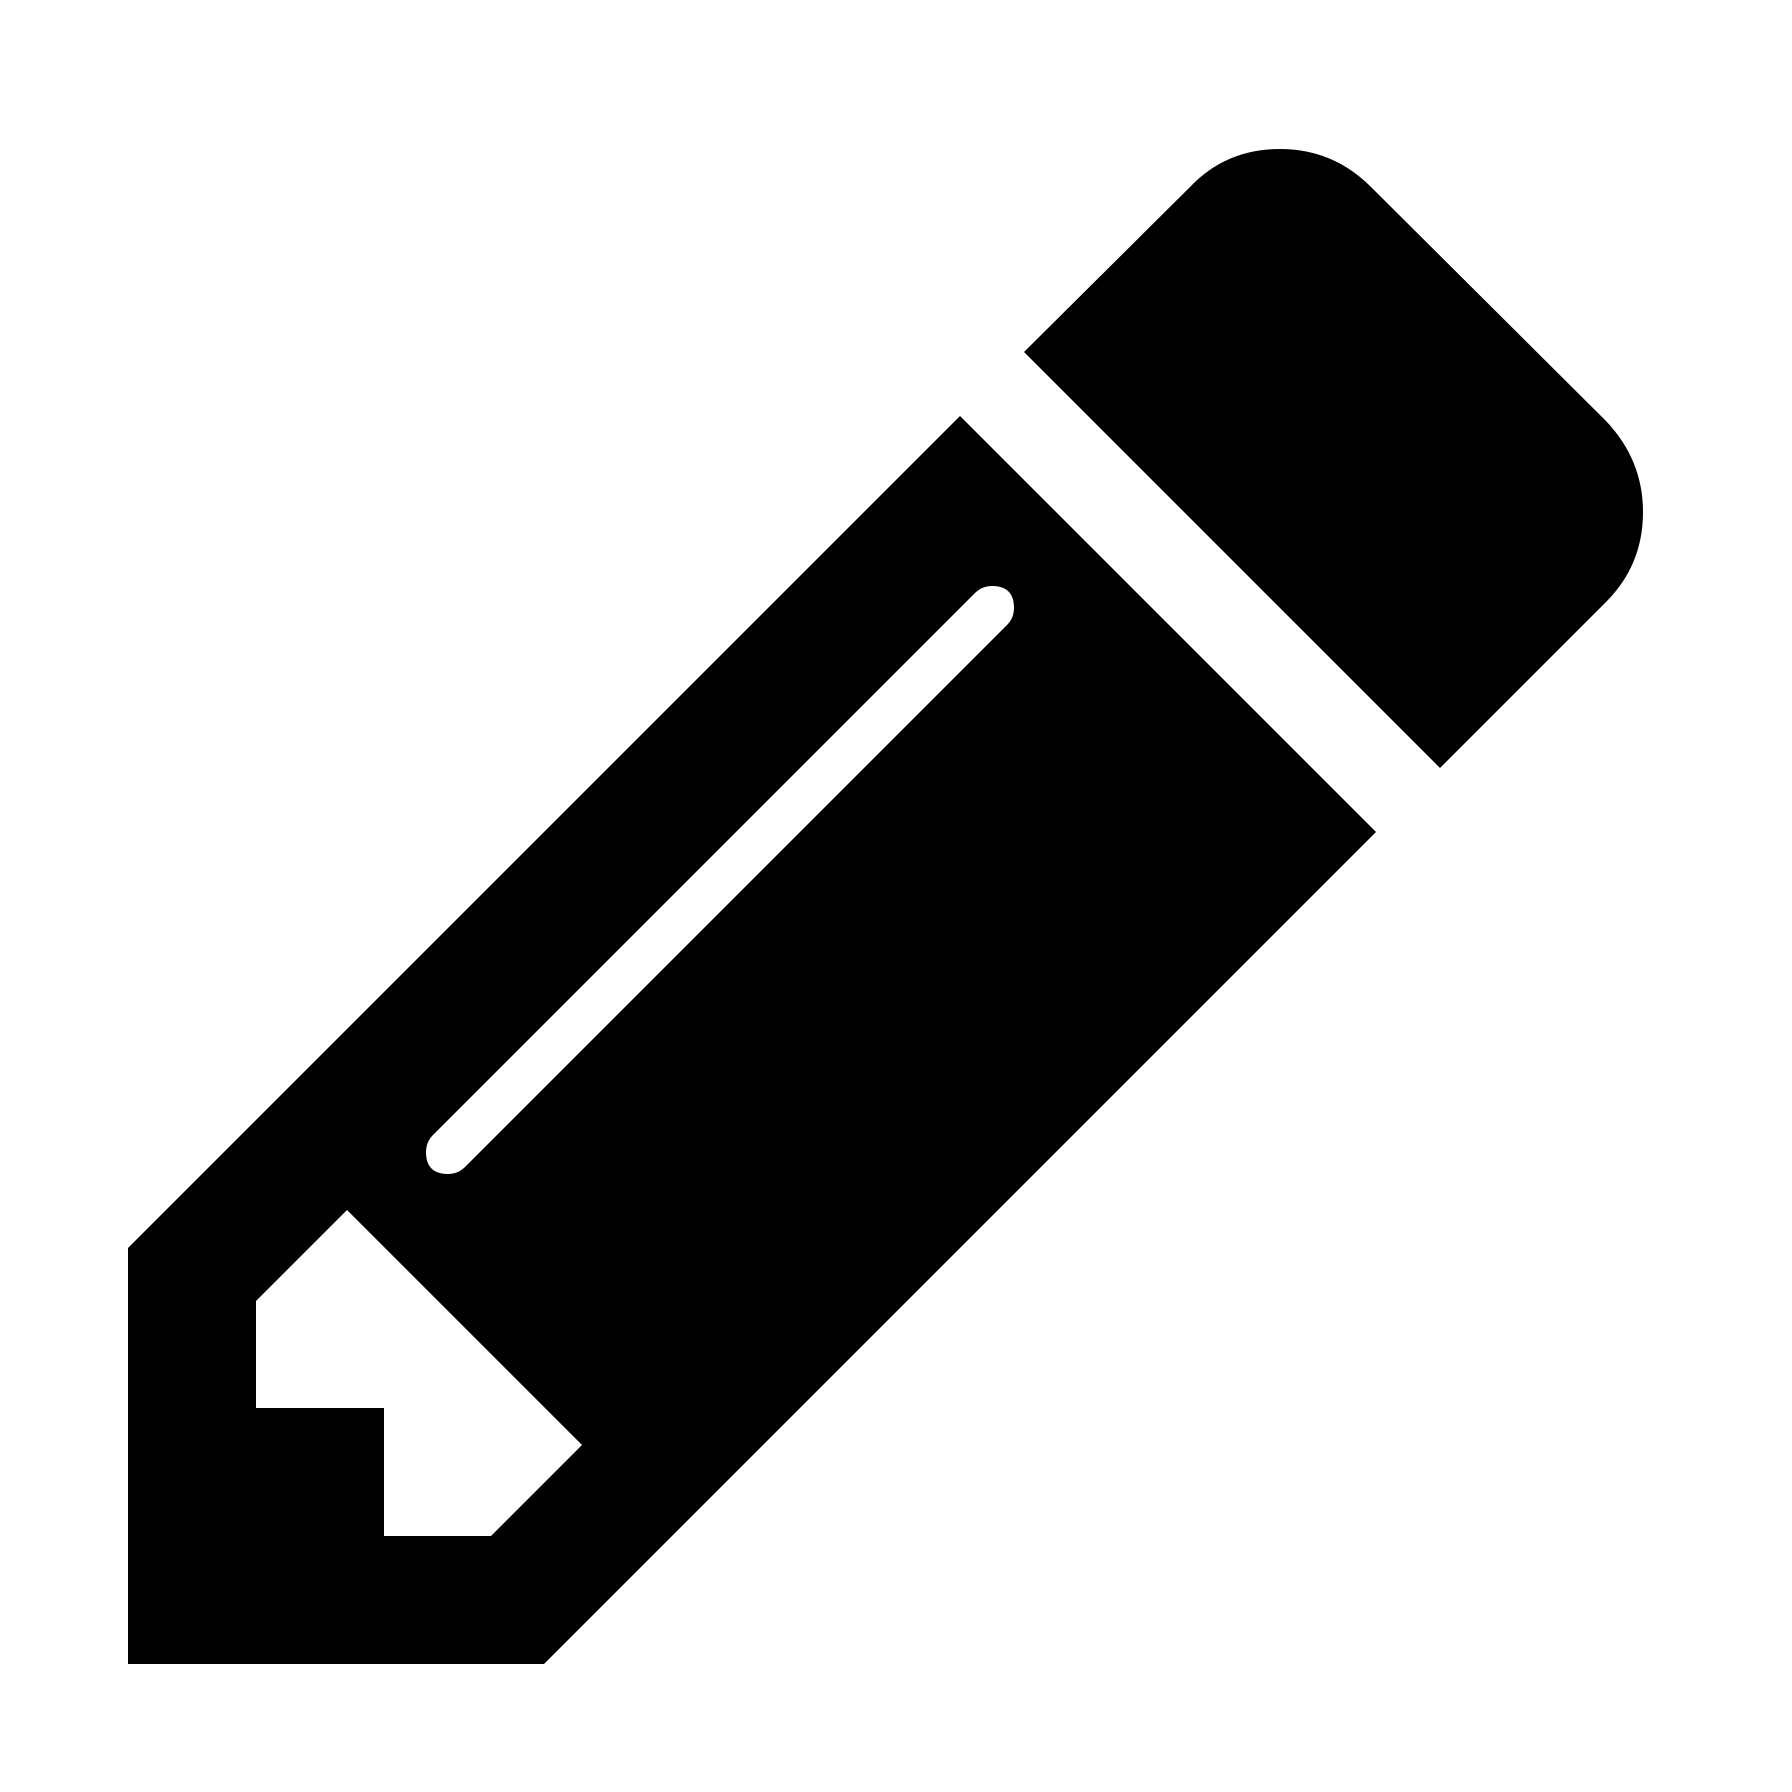
\includegraphics{images/pencil}	\textbf{Catatan} 
	\begin{itemize}
		\item Kata
		kunci virtual tidak membuat metode tersebut harus dioverride.
		\item Pada kelas turunan metode virtual yang dioveride
		otomatis virtual walaupun tidak dtiulis, namun sebaiknya untuk kemudahan
		perawatan sebaiknya kata kunci virtual ditulis.
		\item Variabel pointer bertipe kelas dasar jika digunakan untuk menunjuk objek
		bertipe kelas turunan, untuk mengakses anggota kelas turunannya, ia
		hanya bisa memanggil metode virtual yang dioverride oleh kelas
		turunannya. Dengan kata lain, variabel tersebut tidak bisa memanggil
		metodemetode kelas turunan yang bukan merupakan override dari metode
		virtual kelas dasar.
	\end{itemize}
\end{quotation}
 

\section{Pemotongan (Slicing)}\label{pemotongan-slicing}

Perlu diperhatikan bahwa kemampuan untuk memanggil metode kelas turunan
dari variabel bertipe kelas dasar hanya berlaku untuk variabel pointer
dan variabel referensi, sedangkan variabel nilai (value variable) tidak
dapat mengakses metode virtual seperti itu.

Ketika kita membuat objek bertipe kelas turunan, sebenarnya sebelumnya
sudah dibuat objek bertipe kelas dasarnya, seperti sudah dibahas secara
tidak langsung pada bagian yang membicarakan konstruktor di atas. Jadi
ada bagian yang merupakan anggota kelas dasar dan ada bagaian yang
merupakan anggota kelas turunan. Sebagai contoh misalnya berikut ini
ilustrasi mengenai objek bertipe Silinder yang merupakan turunan dari
kelas Lingkaran yang dibahas pada contoh 10 di atas.

\begin{figure}[htbp]
\centering
\includegraphics[width=0.8\textwidth]{images/capture7-6.png}
\caption{Bagan pemotongan antara lingkaran dan silinder}
\end{figure}

Pada konversi dari suatu variabel ke variabel lain, bisa terjadi
Pemotongan (Silicing). Supaya lebih jelas lakukan percobaan berikut ini.

\subsubsection*{Contoh  Metode virtual dan non virtual.}

Jalankan Qt Console Application projek, buka projek bernama contoh \ref{Metode-virtual-nonvirtual}
yang dibuat tadi, kemudian ubah kode progam pada bagian program utama
seperti berikut:



\begin{lstlisting}[language=c++, caption=Metode virtual dan non virtual]
int main(int argc, char *argv[])
{
QCoreApplication a(argc, argv);
Silinder* s = new Silinder(); //<-- objek bertipe Silinder
Lingkaran* objek1 = s; //<-- variabel pointer bertipe kelas dasar
Lingkaran& objek2 = *s; //<-- variabel referensi bertipe kelas dasar
Lingkaran objek3 = *s; //<-- variabel nilai bertipe kelas dasar
cout << "Pointer : " ;
objek1->getLuas(); //<-- memanggil dai variabel pointer
cout << "Referensi : " ;
objek2.getLuas(); //<-- memanggil dai variabel referensi
cout << "Nilai : " ;
objek3.getLuas(); //<-- memanggil dai variabel nilai
return a.exec();
}
\end{lstlisting}

Tekan Ctrl+R untuk menjalankan program diatas, hasil keluaran adalah
sepeti berikut.

\begin{lcverbatim}
Pointer : Luas Silinder
Referensi : Luas Silinder
Nilai : Luas Lingkaran
\end{lcverbatim}

\textbf{Keterangan:}

\begin{itemize}

\item
  Tampak pada hasil percobaan, pointer dan referensi memanggil metode
  virtual, sehingga yang dieksekusi adalah metode \texttt{getLuas()}
  milik Silinder. Ini tampak pada 2 baris pertama hasil keluaran di
  atas. Sedangkan pada baris ke 3 metode yang dieksekusi adalah metode
  milik kelas dasar (Lingkaran) itu sendiri.
\item
  Variabel objek3 bertipe kelas dasar (Lingkaran), maka ketika menerima
  objek bertipe kelas turunan (Silinder) kompiler memotong (slices down)
  objek Silinder menjadi bentuk kelas dasar (Lingkaran) saja. Oleh
  karena itu ketika dipanggil metode \texttt{getLuas()} maka yang ada
  hanya anggota-anggota kelas dasar (Lingkaran). Potongan objek bertipe
  kelas turunan (Silinder) hilang, inilah efek dari variabel nilai yang
  diberi nilai objek kelas turunannya, efek ini disebut Pemotongan
  (Slicing) karena bagian kelas turunan (Silinder) dipotong keluar
  ketika dikonversikan menjadi kelas dasar (Lingkaran).
\end{itemize}

\section{Memakai static\_cast}\label{memakai-staticux5fcast}

Seperti tertulis pada catatan di atas, pointer bertipe kelas dasar yang
menunjuk objek bertipe kelas turunan tidak bisa memanggil metode-metode
kelas turunan yang bukan merupakan override dari metode virtual kelas
dasar. Namun dengan mekanisme casting hal ini bisa dilakukan.

Casting adalah mekanisme yang digunakan untuk mengubah tipe variabel
dari tipe data ke tipe data yang lain. \texttt{static\_cast} adalah
mekanisme yang dapat digunakan untuk mengkonversikan pointer ke tipe
pointer lain yang mempunyai hubungan kekerabatan (inheritance) dan
melakukan konversi secara ekplisit tipe data standar.
\texttt{static\_cast} pada saat kompilasi melakukan pemeriksaan untuk
memastikan bahwa pointer yang akan di-``cast'' mempunyai hubungan yang
benar. Dengan static\_cast sebuah pointer dapat di-``up-casted'' menjadi
tipe kelas dasar, atau bisa pula di-``down-casted'' menjadi bertipe
kelas turunan. Jika suatu variabel bertipe kelas dasar diberi nilai
objek bertipe kelas turunan sebagai berikut:

\begin{lstlisting}[language=c++, numbers=none]
Kelas_dasar* variabel1 = new Kelas_turunan();
\end{lstlisting}

Maka tipe data variabel tersebut bisa di-``down-casted'' menjadi tipe
data kelas turunan dengan cara:

\begin{lstlisting}[language=c++, numbers=none]
Kelas_turunan* variabel2 = static_cast<Kelas_turunan*>(variabel1);
\end{lstlisting}

\subsubsection*{Contoh  Memakai static\_cast.}

Jalankan Qt Console Application projek, buka projek bernama contoh \ref{Metode-virtual-nonvirtual} di
atas, ubah pada bagian program utama (main()) menjadi seperti berikut:

\begin{lstlisting}[language=c++, caption=Memakai static\_cast]
int main(int argc, char *argv[])
{
QCoreApplication a(argc, argv);
Lingkaran* objek1; //<-- variabel pointer bertipe kelas dasar
objek1 = new Silinder(); //<-- objek bertipe kelas turunan
objek1->getLuas(); //<-- memanggil metode yang dioverride
static_cast<Silinder*>(objek1)->getVolume(); //<-- casting mjd Silinder
return a.exec();
}
\end{lstlisting}

Tekan Ctrl+R untuk menjalankan program diatas, hasil keluaran adalah
sepeti berikut.

\begin{lcverbatim}
Luas Silinder
Volume Silinder
\end{lcverbatim}

\textbf{Keterangan:}

\begin{itemize}

\item
  Tampak pada program utama, variabel pointer bertipe kelas dasar
  (Lingkaran), yaitu K, di-``down-casted'' menjadi tipe data kelas
  turunan (Silinder). Ketika dipanggil metode \texttt{getVolume()} yang
  sebenanya tidak ada di kelas dasar tetapi hanya ada di kelas turunan,
  tampak bahwa metode \texttt{getVolume()} milik kelas Silinder
  menanggapinya.
\item
  Percobaan ini menunjukkan bahwa tipe data pointer dapat dikonversikan
  menjadi tipe data pointer lain.
\end{itemize}

\begin{quotation}
	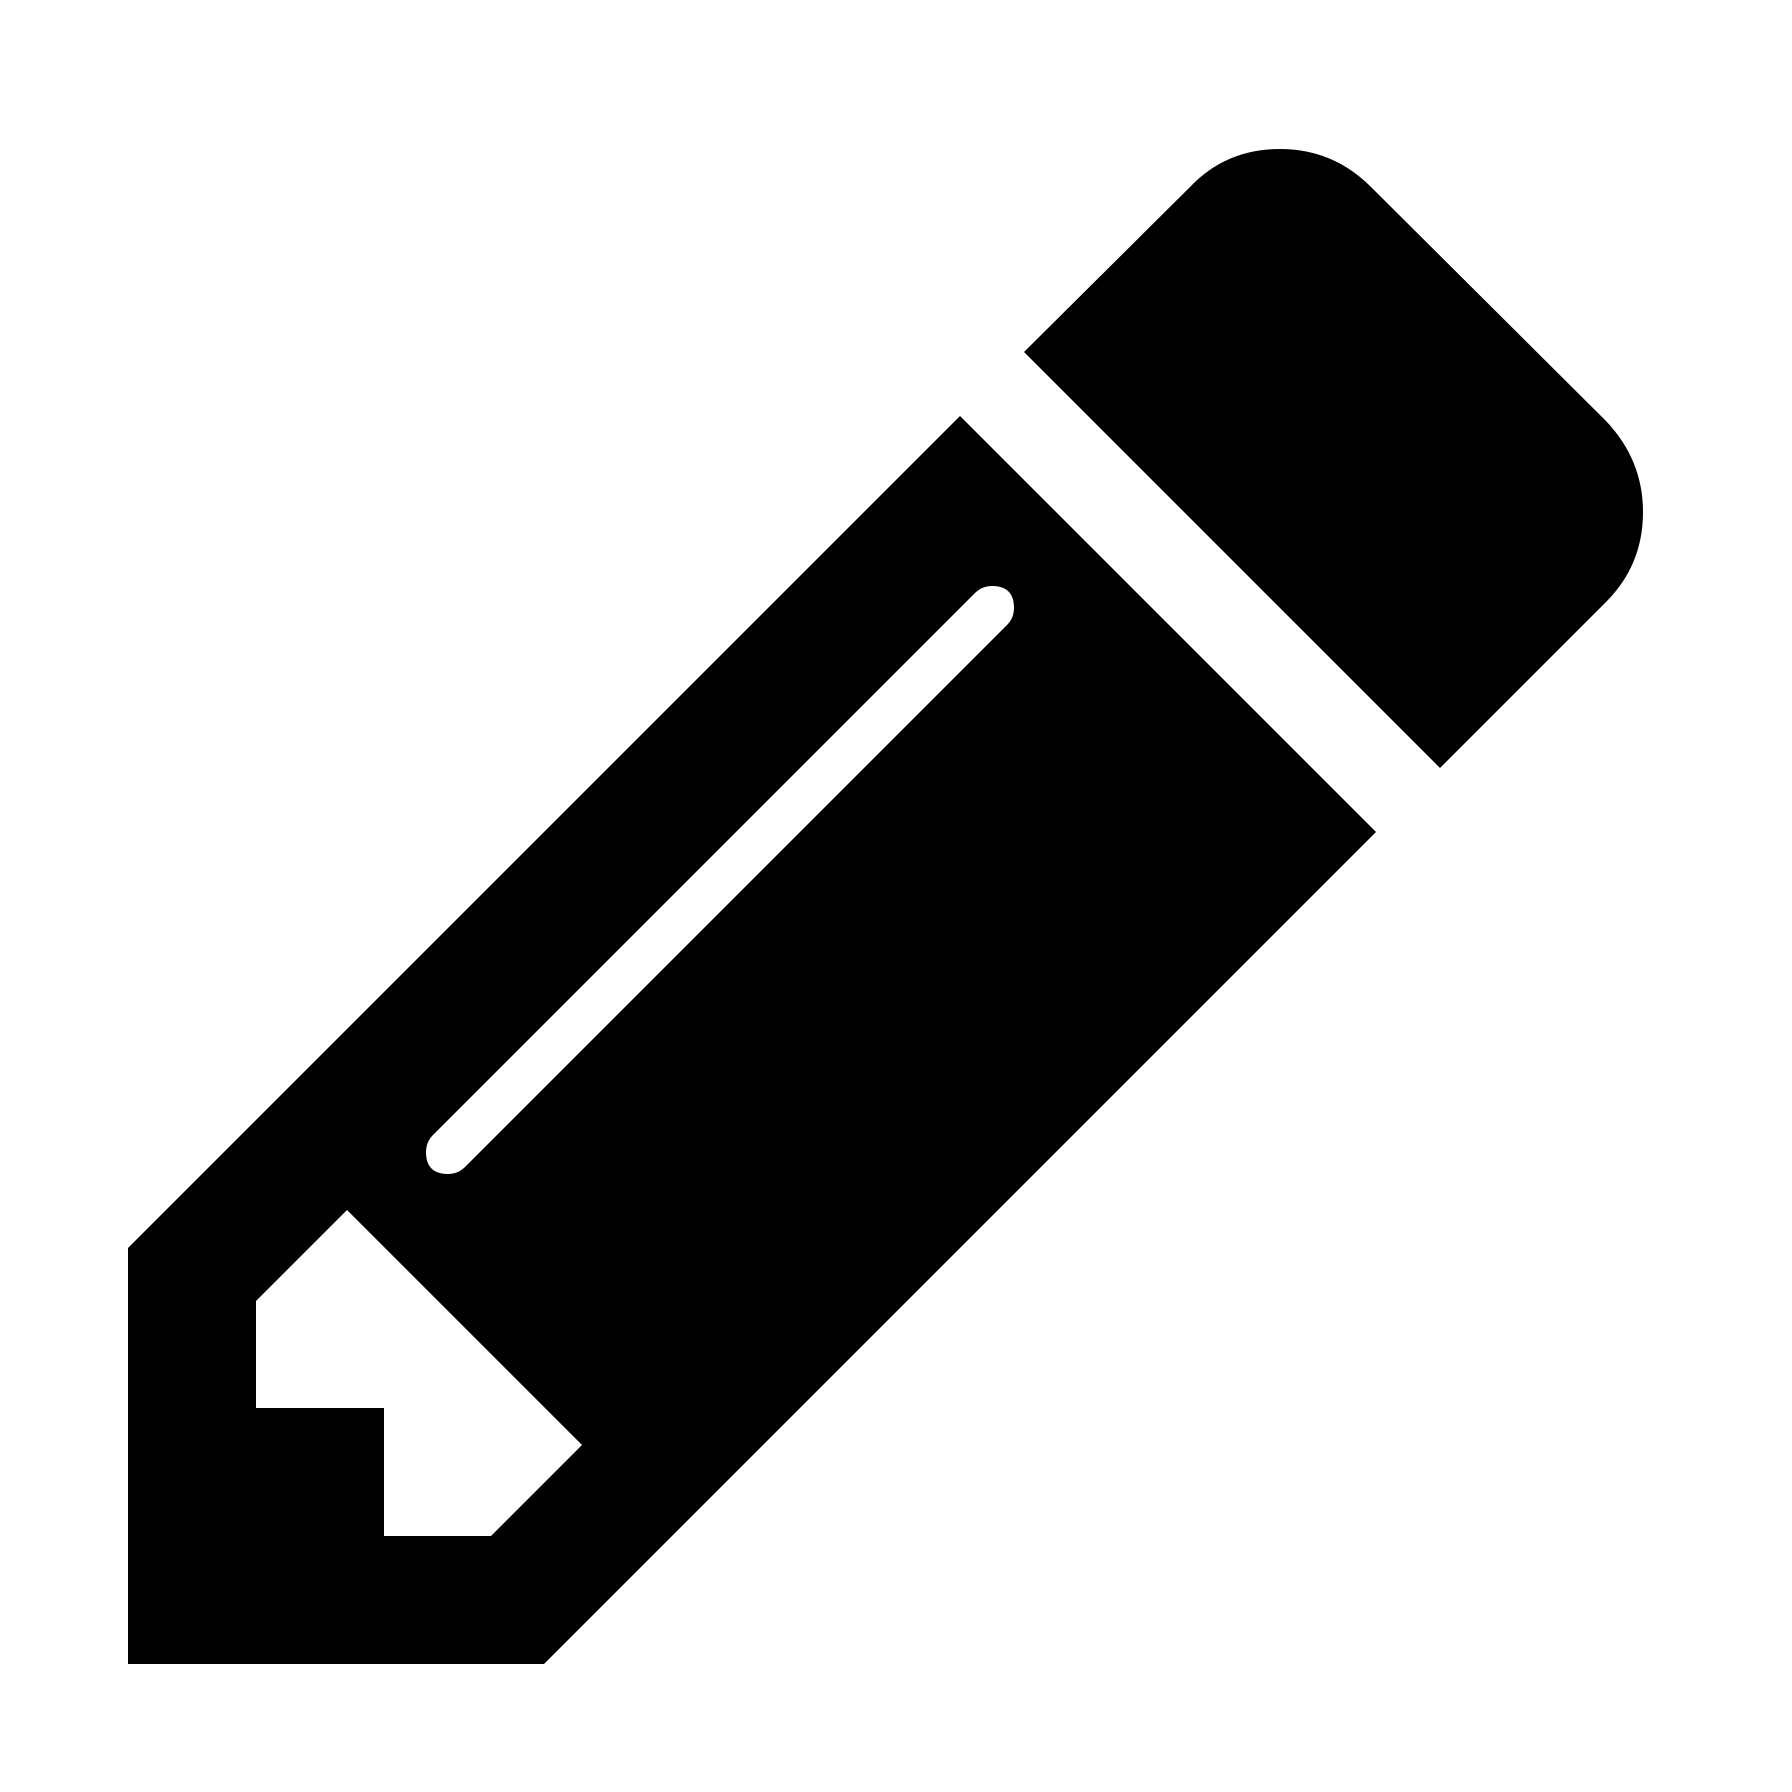
\includegraphics{images/pencil} \textbf{Catatan} 
	\begin{itemize}
		\item Casting terhadap pointer hanya bisa dilakukan terhadap tipe-tipe yang
		mempunyai hubungan kekerabatan (inheritance).
		\item  Dengan
		casting kita bisa memaksa variabel pointer bertipe kelas dasar yang
		digunakan untuk menunjuk objek bertipe kelas turunan untuk memanggil
		metode yang bukan merupakan override dari metode virtual kelas dasar,
		namun cara ini tidak cukup aman jika objek tersebut bukan dari kelas
		turunan.
	\end{itemize}
\end{quotation}


